% witness: arXiv 2605.15377, 2605.22769 (pgf-blur `blur shadow`, tikzlibraryshadows.blur.code.tex:181 a nested \pgfpicture)
% oracle:  pdflatex 0 errors; Perl 0 errors
% engines: rust 56kf (broad route) Fatal PushbackLimit (the nested picture's \pgf@setlength calls itself); 56ke and the
%          typed route 0 errors
% expect:  0 errors, 0 warnings, 0 fatals
% status:  GREEN (the route is taken only for latex.ltx's \setlength operands)
% A nested \pgfpicture saves `\pgf@setlength` as `\pgf@setlengthorig` (pgfcorescopes.code.tex:238-241), so `\setlength`
% there calls itself; TeX never calls it, since `\pgfsetlinewidth` reads through pgfmath (pgfcoregraphicstate.code.tex).
\documentclass{article}
\usepackage{tikz}
\begin{document}
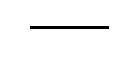
\begin{tikzpicture}
\pgfpicture\pgfsetlinewidth{1pt}\pgfpathmoveto{\pgfpointorigin}\pgfpathlineto{\pgfpoint{1cm}{0cm}}\pgfusepath{stroke}\endpgfpicture
\end{tikzpicture}
\end{document}
